
\section{Deviations from the registered plan}
\label{app:deviations}

Table~\ref{tab:deviations} lists every place where the analysis could not follow \texttt{preregistration/protocol-stage2.md} (tag \texttt{prereg-v2.1}) as written.
The changes made after the pilot and before the registration are part of the registered plan (its section 10) and are not repeated here.

\begin{table*}[t]
  \centering
  \small
  \begin{adjustbox}{max width=\linewidth}
  \begin{tabular}{@{}p{0.30\textwidth}p{0.64\textwidth}@{}}
    \toprule
    Registered & What was done \\
    \midrule
    Matcher thresholds frozen and tagged \texttt{scorer-v1} before study outputs are scored (5.2) & The matcher was frozen with the registered plan (tag \texttt{prereg-v2.1}) instead of under a separate tag, and scores the study unchanged. \\
    Five matcher labels (5.2, 5.3 b) & The matcher does not assign ``true item the list missed'' or ``text from beyond the excerpt''; those entries land in ``wrong kind'' or ``invented''. Their places in the 400-entry draw go in equal parts to the other three labels (134, 133, 133), as 5.3 b allows for a label with too few entries. \\
    Scoring check on 40 pilot outputs before the full run (5.3 a) & Drawn as registered and done during the full run rather than before it (65 replies: 40 random, 3 cut at the token limit, 22 unreadable). No scorer bug was found (Appendix~\ref{app:checks}). \\
    Escape outcome ``extra entries per padded slot'' (6.2, contrast 5) & Computed per output as excess / ($k - n$), the slots the grammar forces beyond the true items; this paper calls them forced slots. \\
    Poisson mixed model for contrast 5 (6.2) & A variational-Bayes fit with a random intercept per document and $\log(k - n)$ as a covariate, reported as a rate ratio next to the primary bootstrap test. \\
    Mixed models of the paired difference (6.2) & Covariates centred and factors sum-coded, so the intercept is the average paired difference; the intercept and its Wald interval are reported. \\
    ``Says it is short'' from notes outside the list (5.2) & The frozen note rules applied to each sentence outside the JSON; notes they do not cover are missed, so the share is a lower bound. \\
    $n = 0$ analysed apart (6.1) & The primary contrasts pool every $n < k$ cell, as the pilot's stop rules did; $n = 0$ and $n \geq 1$ are given separately (Appendix~\ref{app:key}). \\
    Same-weights pairs, ``10 points'' (3.3) & The rule was written for over-count; the pair table gives length and over-count and judges the rule on over-count points. \\
    400-entry frame: every substantive entry of every study output (5.3 b) & The frame leaves out the thinking-pair runs, which finished after the draw was fixed. \\
    RQ5, RQ7, RQ8 and the robustness arms (2, 3.2) & The teacher-forced and hidden-state analyses are left to future work; the robustness arms ran in the pilot. \\
    Every request answered (9) & 11 outputs are missing after repeated transport errors (Qwen3.5-0.8B 1, Qwen3.5-2B 3, gpt-oss-20b 6) or timeouts (Gemma 4 31B with thinking on, 1); they are left out of every pair. \\
    \bottomrule
  \end{tabular}
  \end{adjustbox}
  \caption{Deviations from the registered plan (protocol section in brackets).}
  \label{tab:deviations}
\end{table*}

\section{The authors' checks}
\label{app:checks}

The protocol registers three checks by the authors (section 5.3); their sheets were drawn with a fixed seed by committed scripts (\texttt{analysis/full\_study\_sheets.py}, \texttt{analysis/human/}).

\paragraph{(a) Scoring check.}
One author reads 65 pilot replies (40 drawn at random, the 3 outputs cut at the token limit and all 22 unreadable ones) against the scorer: parse rung, substantive entries, placeholders, repeats, over-count.
The author and the scorer agree fully on 61 of the 65.
The 4 differences all come from how the frozen scorer reads an output.
In one, the author counts as a repeat an entry that restates an earlier one with a three-word prefix; the scorer counts as repeats only entries with the same or nearly the same words (overlap threshold 0.85, here 0.67) and leaves the rest to the matcher.
In three, the reply is cut at the token limit inside an entry; the author counts the unfinished entry and the scorer keeps only entries that close before the cut, so in one of them the author sees an over-count the scorer does not.
No scorer bug was found, so nothing is rescored.

\paragraph{(b) Matcher labels.}
The matcher matches names after normalising case and punctuation, quotes by fuzzy substring search, and meeting action items by similarity to each answer item and its transcript lines.
Both authors label 400 entries alone, blind to the model, condition, $k$, the other entries and the matcher's label, then settle the differences.
They chose the same label for 370 of the 400 entries (92.5\%; Cohen's kappa 0.896, Gwet's AC1 0.912) and settled the other 30 together; the settled label is the reference.
Table~\ref{tab:matchercheck} gives the matcher against it.
The matcher gave no study entry the labels ``true item the list missed'' or ``text from beyond the excerpt'', so those strata are empty and their places went to the other three.
The invented share of substantive entries is 7.0\% as the matcher gives it and 7.3\% weighted by the authors' labels.
Five entries were settled as true items the list missed; they go into the answer-list overlay with the document's wording and the authors' reason (\texttt{analysis/gold\_overlay.jsonl}; the one review item's text is in the local restricted file), and with the overlay applied contrasts 1 to 4 are the same to two decimals and contrast 2 on over-count moves from $+20.9$ to $+21.1$ points.

\begin{table*}[t]
  \centering
  \small
  \begin{tabular}{@{}lrrrcc@{}}
    \toprule
    Matcher label & Frame entries & Drawn & Used & Precision [95\% CI] & Recall [95\% CI] \\
    \midrule
    True item or split & 637,844 & 134 & 134 & 0.98 [0.95, 1.00] & 0.94 [0.90, 0.97] \\
    Wrong kind & 408,859 & 133 & 133 & 0.85 [0.78, 0.91] & 0.96 [0.93, 0.99] \\
    Invented & 78,798 & 133 & 131 & 0.69 [0.56, 0.83] & 0.66 [0.53, 0.83] \\
    \bottomrule
  \end{tabular}
  \caption{The matcher against the authors' settled labels of 400 entries. Precision: share of the matcher's calls the authors confirm. Recall: share of the authors' labels the matcher finds, each stratum weighted back to its size in the frame. Intervals: 10,000 bootstrap draws over document groups. Used: entries whose settled label is not ``unsure''; the two left out are clinical entries saying no medication was given, which the authors settled as unsure.}
  \label{tab:matchercheck}
\end{table*}

\paragraph{(c) Hand recount.}
For 10 documents with $n < k$, each paired with one GPU model, one author counts the substantive entries of 7 outputs by hand (70 outputs) and computes length change, over-count, true items left out and the sorting.
The hand count agrees fully with the scorer on 60 of the 70.
In 7 (Qwen3.5-0.8B on one email), the model wrote its list inside a copy of the schema; the frozen parser counts that as unreadable with 0 entries while the author reads the list, and three length changes follow from it.
In 3 (gpt-oss-20b on one meeting), the matcher matched an entry naming another task or person to the one true item on shared words, so the scorer counts no true item left out and the author counts one; the author is right, and this is the kind of error check (b) measures.

\section{Data, models and licences}
\label{app:data}

Table~\ref{tab:licences} lists the nine sets with their sources and licences, and Table~\ref{tab:models} the models with their pinned revisions, requests and compute.

\begin{table*}[t]
  \centering
  \small
  \begin{adjustbox}{max width=\linewidth}
  \begin{tabular}{@{}lllll@{}}
    \toprule
    Set & One document is & Item type & Source dataset & Licence \\
    \midrule
    meetings & a window of a meeting transcript & summary sentence & AMI Meeting Corpus \citep{carletta2005ami} & CC BY 4.0 \\
    emails & one Enron email & exact quote & MailEx \citep{srivastava2023mailex} & CC BY-SA 4.0 \\
    receipts & one receipt as plain text & name & CORD v2 \citep{park2019cord} & CC BY 4.0 \\
    job-ad skills & 4--10 sentences of a job ad & exact quote & SkillSpan \citep{zhang2022skillspan} & CC BY 4.0; TECH ads CC BY-SA \\
    clinical & 3--8 sentences of a case report & name & MACCROBAT2020 \citep{caufield2019maccrobat} & CC BY 4.0 \\
    reviews & one product or service review & exact quote & ROAST \citep{roast} & Apache-2.0 (annotations) \\
    job-ad knowledge & 4--10 sentences of a job ad & name & SkillSpan & CC BY 4.0; TECH ads CC BY-SA \\
    Wikipedia people & one Wikipedia sentence & name & Few-NERD \citep{ding2021fewnerd} & CC BY-SA 4.0 \\
    novel quotes & 1--3 paragraphs of a novel & exact quote & PDNC \citep{vishnubhotla2022pdnc} & CC BY 4.0 \\
    \bottomrule
  \end{tabular}
  \end{adjustbox}
  \caption{The nine sets and their sources. SkillSpan's release is CC BY 4.0, but its paper states that the TECH job ads, from Stack Overflow, are CC BY-SA (71 of the 127 job-ad documents). Review text is not redistributed; those documents are rebuilt locally from the source.}
  \label{tab:licences}
\end{table*}

\begin{table*}[t]
  \centering
  \small
  \begin{adjustbox}{max width=\linewidth}
  \begin{tabular}{@{}lll@{}}
    \toprule
    Model & Served as & Revision or model id \\
    \midrule
    Qwen3.5-0.8B & GPU, vLLM & \texttt{Qwen/Qwen3.5-0.8B} @ \texttt{2fc06364715b} \\
    Qwen3.5-2B & GPU, vLLM & \texttt{Qwen/Qwen3.5-2B} @ \texttt{15852e8c1636} \\
    Qwen3.5-9B & GPU, vLLM & \texttt{Qwen/Qwen3.5-9B} @ \texttt{c20223623576} \\
    Qwen3.5-27B & GPU, vLLM & \texttt{Qwen/Qwen3.5-27B} @ \texttt{fc05daec18b0} \\
    Gemma 4 31B & GPU, vLLM & \texttt{google/gemma-4-31B-it} @ \texttt{842da3794eaa} \\
    Olmo 3.1 32B & GPU, vLLM & \texttt{allenai/Olmo-3.1-32B-Instruct} @ \texttt{ac0587e4a774} \\
    Ministral 3 14B & GPU, vLLM & \texttt{mistralai/Ministral-3-14B-Instruct-2512-BF16} @ \texttt{3cea74c1ebaf} \\
    gpt-oss-20b & GPU, vLLM & \texttt{openai/gpt-oss-20b} @ \texttt{6cee5e81ee83} \\
    \midrule
    DeepSeek V4.1 Flash & Together, every condition & \texttt{deepseek-ai/DeepSeek-V4.1-Flash} \\
    Qwen3.5-9B & Together, every condition & \texttt{Qwen/Qwen3.5-9B} \\
    Kimi K3 & Bedrock, prompt-side & \texttt{us.moonshotai.kimi-k3} \\
    DeepSeek V3.2 & Bedrock, prompt-side & \texttt{deepseek.v3.2} \\
    Qwen3-235B & Bedrock, prompt-side & \texttt{qwen.qwen3-235b-a22b-2507-v1:0} \\
    Mistral Large 3 & Bedrock, prompt-side & \texttt{mistral.mistral-large-3-675b-instruct} \\
    gpt-oss-120b & Bedrock, prompt-side & \texttt{openai.gpt-oss-120b-1:0} \\
    Ministral 3 14B & Bedrock, prompt-side & \texttt{mistral.ministral-3-14b-instruct} \\
    gpt-oss-20b & Bedrock, prompt-side & \texttt{openai.gpt-oss-20b-1:0} \\
    \bottomrule
  \end{tabular}
  \end{adjustbox}
  \caption{Models. GPU models are pinned to a Hugging Face revision (first 12 characters shown); hosted models are named by the service's model id and pin no revision. GPU and Together models have 26,784 request ids each and Bedrock models 23,436; the no-count prompt answers its ids at all three $k$, so 25,668 and 22,320 prompts are sent. The GPU models ran on one NVIDIA RTX PRO 6000 Blackwell (96 GB): about 31 GPU hours for the full study and 3 h 52 min for the pilot. Hosted inference cost about 6.63 USD on Together AI for the full study and 3.64 USD for the pilot, and about 58.80 USD on Amazon Bedrock.}
  \label{tab:models}
\end{table*}

\section{Answer key, $n = 0$ and generality}
\label{app:key}
\label{app:generality}

\paragraph{Blind check.}
On 40 documents from eight sets, each author counted the items alone, without seeing the answer lists.
Author A matched the list's count on 35 (87.5\%; 95\% Wilson interval 74 to 95\%), author B on 38 (95.0\%), and A and B agreed on 35 (AC1 0.851), passing the registered thresholds of 85\% and 0.80; 15 of the 40 were marked unclear by either author.
Per set (5 documents each; A matches, B matches, A = B): clinical, emails and job-ad knowledge 5, 5, 5; novel quotes, receipts and Wikipedia people 5, 5, 5; meetings 3, 5, 3; job-ad skills 2, 3, 2.
Before the first plan was frozen, an earlier round under one-line item definitions (A 72.5\%, B 65.0\%) showed which counting rules the definitions left unstated; five definitions were extended to state them, and the registered check uses the final definitions: 25 fresh documents of the five extended sets and 15 earlier documents of the three unchanged ones.
No answer list was changed after the check.
The reviews set, whose text may not be shared, was counted the same way in a separate check of five documents: author A matched the list on all five, author B on four, and the two agreed on four.
Both authors read the 60 pilot documents with their lists during the cleanup review.

\begin{table}[t]
  \centering
  \small
  \begin{adjustbox}{max width=\linewidth}
  \begin{tabular}{@{}lrrrr@{}}
    \toprule
    Set & Docs & Same & Higher & Lower \\
    \midrule
    meetings & 70 & 44 & 22 & 4 \\
    emails & 61 & 39 & 4 & 18 \\
    receipts & 55 & 55 & 0 & 0 \\
    job-ad skills & 70 & 55 & 15 & 0 \\
    clinical & 70 & 55 & 1 & 14 \\
    reviews & 55 & 21 & 9 & 25 \\
    job-ad knowledge & 57 & 46 & 5 & 6 \\
    Wikipedia people & 60 & 49 & 3 & 8 \\
    novel quotes & 60 & 59 & 0 & 1 \\
    \bottomrule
  \end{tabular}
  \end{adjustbox}
  \caption{Cleaned answer lists against the source datasets' own counts: documents whose cleaned count is the same, higher or lower.}
  \label{tab:keysource}
\end{table}

\begin{table*}[t]
  \centering
  \small
  \begin{adjustbox}{max width=\linewidth}
  \begin{tabular}{@{}lrrrrr@{}}
    \toprule
     & Frozen lists & Annotators' counts & List kept & List changed & Overlay \\
    \midrule
    \rows{generated/app_key_variants_rows.tex}
    \bottomrule
  \end{tabular}
  \end{adjustbox}
  \caption{Contrasts 1 to 4 (entries) with the answer-key variants of protocol 4.2 and 4.3. The annotators' counts change only which documents are in the $n < k$ cells. List kept and list changed split the documents by whether the cleanup changed their answer list. The overlay applies the authors' 5 corrections (Appendix~\ref{app:checks}). Contrast 2 on over-count: frozen $+20.9$ [19.5, 22.3], annotators' counts $+19.3$ [17.9, 20.7], overlay $+21.1$ [19.6, 22.6].}
  \label{tab:keyvariants}
\end{table*}

\begin{table}[t]
  \centering
  \small
  \begin{adjustbox}{max width=\linewidth}
  \begin{tabular}{@{}lrr@{}}
    \toprule
     & $n = 0$ & $n = 1$ to 4, $n < k$ \\
    \midrule
    \rows{generated/app_n0_rows.tex}
    \bottomrule
  \end{tabular}
  \end{adjustbox}
  \caption{Confirmatory contrasts with $n = 0$ apart from $n \geq 1$ (protocol 6.1).}
  \label{tab:n0}
\end{table}

\paragraph{Generality (contrast 2).}
\begin{itemize}
  \setlength\itemsep{0pt}
    \item models whose own interval is above 0: 6 of 8 (Qwen3.5-9B, Qwen3.5-27B, Gemma 4 31B, Olmo 3.1 32B, Ministral 3 14B, gpt-oss-20b)
  \item the 5 families weighted equally (gemma, gpt-oss, mistral, olmo, qwen; within a family its models equally): +0.72 [+0.62, +0.81]
  \item leaving out gemma: +0.47 [+0.29, +0.65]
  \item leaving out gpt-oss: +0.59 [+0.40, +0.77]
  \item leaving out mistral: +0.67 [+0.48, +0.85]
  \item leaving out olmo: +0.67 [+0.49, +0.85]
  \item leaving out qwen: +0.78 [+0.69, +0.86]

\end{itemize}

\section{Pooled confirmatory tests and per set}
\label{app:perset}

Table~\ref{tab:confirmatory} gives the five confirmatory contrasts pooled with their tests, Table~\ref{tab:perset} gives them per set, and Table~\ref{tab:wordings} gives each prose wording.

\begin{table*}[t]
  \centering
  \small
  \begin{adjustbox}{max width=\linewidth}
  \begin{tabular}{@{}lrrrrr@{}}
    \toprule
    \# & Estimate [95\% CI] & $p$ & Holm $p$ & Pairs & Groups \\
    \midrule
    \rows{generated/app_confirmatory_a_rows.tex}
    \bottomrule
  \end{tabular}
  \end{adjustbox}

  \vspace{6pt}
  \begin{adjustbox}{max width=\linewidth}
  \begin{tabular}{@{}lrrr@{}}
    \toprule
    \# & Without pilot documents & Mixed model & Over-count (points) \\
    \midrule
    \rows{generated/app_confirmatory_b_rows.tex}
    \bottomrule
  \end{tabular}
  \end{adjustbox}
  \caption{Confirmatory contrasts, eight GPU models pooled, documents with $n < k$, $k = 3$ and 5. C1 to C4 in entries, C5 in excess entries per forced slot. Mixed model (statsmodels \texttt{MixedLM}; for C5 \texttt{PoissonBayesMixedGLM}): C1 to C4 the intercept of a linear mixed model of the paired difference ($\sim n$ + model + set + words + (1 $\mid$ document)); C5 the rate ratio of the escape in a Poisson mixed model. Pairs: model--document--$k$ pairs (C1: model--document pairs); groups: the document groups the bootstrap resamples.}
  \label{tab:confirmatory}
\end{table*}

\begin{table*}[t]
  \centering
  \small
  \begin{adjustbox}{max width=\linewidth}
  \begin{tabular}{@{}lrrr@{}}
    \toprule
    Set & C1 & C2 & C3 \\
    \midrule
    \rows{generated/app_perset_a_rows.tex}
    \bottomrule
  \end{tabular}
  \end{adjustbox}
  \hfill
  \begin{adjustbox}{max width=\linewidth}
  \begin{tabular}{@{}lrrr@{}}
    \toprule
    Set & C4 & C5 & C2 over-count (pts) \\
    \midrule
    \rows{generated/app_perset_b_rows.tex}
    \bottomrule
  \end{tabular}
  \end{adjustbox}
  \caption{Confirmatory contrasts per set, eight GPU models pooled: C1 to C4 in entries, C5 in excess entries per forced slot, the last column in over-count points. Job-ad skills is the least certain answer list.}
  \label{tab:perset}
\end{table*}

\begin{table}[t]
  \centering
  \small
  \setlength{\tabcolsep}{3pt}
  \begin{adjustbox}{max width=\linewidth}
  \begin{tabular}{@{}lrr@{}}
    \toprule
    Wording (emails) & vs \cnd{none} & Over-count \% \\
    \midrule
    \rows{generated/app_wordings_text_rows.tex}
    \bottomrule
  \end{tabular}
  \end{adjustbox}
  \caption{Prose wordings, shown for emails (other sets name their own item), with the length change against \cnd{none} (entries) and over-count, pooled over all sets and the eight GPU models, $n < k$, $k = 3$ and 5. The schema conditions use ``List all the requests.'' (the escape and ``fewer is fine'' add their line). Templates and the real prompts they are modelled on: \texttt{data/wordings.yaml}.}
  \label{tab:wordings}
\end{table}

\section{Named tests per model}
\label{app:named}

\begin{table*}[t]
  \centering
  \small
  \begin{adjustbox}{max width=\linewidth}
  \begin{tabular}{@{}lrrr@{}}
    \toprule
    Model & \cnd{fewer\_ok} vs \cnd{none} & \cnd{fewer\_ok} vs \cnd{min\_k\_shown} & \cnd{max\_k\_shown} vs \cnd{none} \\
    \midrule
    \rows{generated/app_named_per_model_a_rows.tex}
    \bottomrule
  \end{tabular}
  \end{adjustbox}

  \vspace{6pt}
  \begin{adjustbox}{max width=\linewidth}
  \begin{tabular}{@{}lrrr@{}}
    \toprule
    Model & $n \geq k$: shown vs \cnd{none} & $n < k$ minus $n \geq k$ ($k = 3, 5$) & Empty, $k = 1$: shown vs \cnd{none} (pts) \\
    \midrule
    \rows{generated/app_named_per_model_b_rows.tex}
    \bottomrule
  \end{tabular}
  \end{adjustbox}
  \caption{Named tests per GPU model (entries unless marked).}
  \label{tab:namedpermodel}
\end{table*}

By $k$, the shown minimum against no count on documents with $n \geq k$ is $-0.08$ [$-0.20$, $+0.04$] at $k = 1$, $-0.25$ [$-0.51$, $+0.01$] at $k = 3$ and $-0.71$ [$-1.57$, $-0.02$] at $k = 5$; on $n < k$ it is $+0.22$, $+0.28$ and $+0.86$, and the differences ($n < k$ minus $n \geq k$) are $+0.30$ [$-0.06$, $+0.68$], $+0.54$ [0.20, 0.87] and $+1.57$ [0.84, 2.58].

\section{Outcomes per condition and model}
\label{app:outcomes}

Tables~\ref{tab:outcomes} and~\ref{tab:outcomespooled} give the outcomes by condition, pooled; the tables after them give the same per model, and Table~\ref{tab:unreadable} counts the unreadable outputs.

\begin{table*}[t]
  \centering
  \small
  \begin{adjustbox}{max width=\linewidth}
  \begin{tabular}{@{}lrrrrrrrr@{}}
    \toprule
     & \multicolumn{4}{c}{Sorting, $n < k$ (\%)} & \multicolumn{3}{c}{Length against $k$, $n < k$ (\%)} & Left out\pre{} \\
    \cmidrule(lr){2-5}\cmidrule(lr){6-8}
    Condition & padded & says short & short, no note & unreadable & fewer than $k$ & exactly $k$ & more than $k$ & (\%, $n \geq 1$) \\
    \midrule
    \rows{generated/tab_outcomes_rows.tex}
    \bottomrule
  \end{tabular}
  \end{adjustbox}
  \caption{What the outputs are, by condition, eight GPU models pooled, $k = 3$ and 5. Padded outputs have more substantive entries than $n$; this wins over a note. Left out: share of the true items of documents with $n \geq 1$ that no entry matches. Per model: Tables~\ref{tab:outcomesqwen} and~\ref{tab:outcomesother}.}
  \label{tab:outcomes}
\end{table*}

\begin{table*}[t]
  \centering
  \small
  \begin{adjustbox}{max width=\linewidth}\begin{tabular}{lrrrrrr}
  \toprule
  Condition & Over-count \% & Bound \% & Excess & Unreadable \% & Exactly $k$ \% & Left out \% \\
  \midrule
  \cnd{none} & 34.5 & 34.3 & 2.41 & 6.9 & 5.6 & 17.0 \\
  \cnd{prose\_up\_to\_k} & 42.7 & 42.4 & 1.58 & 3.7 & 24.0 & 20.0 \\
  \cnd{prose\_exactly\_k} & 50.9 & 50.6 & 1.71 & 6.0 & 39.0 & 21.6 \\
  \cnd{max\_k\_shown} & 35.7 & 35.5 & 1.92 & 7.3 & 15.5 & 20.9 \\
  \cnd{min\_k\_shown} & 55.4 & 55.2 & 3.02 & 10.5 & 35.5 & 18.2 \\
  \cnd{min\_k\_shown\_fewer\_ok} & 31.0 & 30.8 & 1.76 & 7.3 & 15.0 & 24.3 \\
  \cnd{min\_k\_enforced} & 90.1 & 89.5 & 3.49 & 0.2 & 71.8 & 8.6 \\
  \cnd{min\_k\_escape} & 51.0 & 50.6 & 2.00 & 0.1 & 78.5 & 13.6 \\
  \bottomrule
\end{tabular}
\end{adjustbox}
  \caption{Over-count, its placeholder bound (every substantive entry of 8 words or fewer holding ``no'', ``none'', ``not'', ``only'', ``other'', ``additional'' or ``found'' taken as a note), mean excess, unreadable share, exactly $k$, on $n < k$, and true items left out\pre{} on $n \geq 1$, eight GPU models pooled, $k = 3$ and 5.}
  \label{tab:outcomespooled}
\end{table*}

\begin{table*}[p]
  \centering
  \small
  \setlength{\tabcolsep}{4pt}
  \begin{adjustbox}{max width=\linewidth}
  \begin{tabular}{@{}lrrrrrrrrrr@{}}
    \toprule
    Condition & Outputs & Over \% & Bound \% & Excess & Unread. \% & $< k$ \% & $= k$ \% & $> k$ \% & $= n$ \% & Left out\pre{} \% \\
    \midrule
    \rows{generated/app_outcomes_grouped_a_rows.tex}
    \bottomrule
  \end{tabular}
  \end{adjustbox}
  \caption{Per GPU model (Qwen3.5 sizes): outputs on $n < k$, over-count, placeholder bound, excess, unreadable, fewer than $k$, exactly $k$, more than $k$, exactly $n$ (all on $n < k$), and true items left out on $n \geq 1$.}
  \label{tab:outcomesqwen}
\end{table*}

\begin{table*}[p]
  \centering
  \small
  \setlength{\tabcolsep}{4pt}
  \begin{adjustbox}{max width=\linewidth}
  \begin{tabular}{@{}lrrrrrrrrrr@{}}
    \toprule
    Condition & Outputs & Over \% & Bound \% & Excess & Unread. \% & $< k$ \% & $= k$ \% & $> k$ \% & $= n$ \% & Left out\pre{} \% \\
    \midrule
    \rows{generated/app_outcomes_grouped_b_rows.tex}
    \bottomrule
  \end{tabular}
  \end{adjustbox}
  \caption{As Table~\ref{tab:outcomesqwen}, for Gemma 4 31B, Olmo 3.1 32B, Ministral 3 14B and gpt-oss-20b.}
  \label{tab:outcomesother}
\end{table*}

\begin{table}[t]
  \centering
  \small
  \setlength{\tabcolsep}{3pt}
  \begin{adjustbox}{max width=\linewidth}
  \begin{tabular}{@{}lrrrr@{}}
    \toprule
    Condition & Padded & Says short & Short, no note & Unread. \\
    \midrule
    \rows{generated/app_sorting_grouped_a_rows.tex}
    \bottomrule
  \end{tabular}
  \end{adjustbox}
  \caption{Sorting per GPU model (\%), Qwen3.5 sizes, selected conditions, $n < k$, $k = 3$ and 5.}
  \label{tab:sortqwen}
\end{table}

\begin{table}[t]
  \centering
  \small
  \setlength{\tabcolsep}{3pt}
  \begin{adjustbox}{max width=\linewidth}
  \begin{tabular}{@{}lrrrr@{}}
    \toprule
    Condition & Padded & Says short & Short, no note & Unread. \\
    \midrule
    \rows{generated/app_sorting_grouped_b_rows.tex}
    \bottomrule
  \end{tabular}
  \end{adjustbox}
  \caption{As Table~\ref{tab:sortqwen}, for the other four GPU models.}
  \label{tab:sortother}
\end{table}

\begin{table*}[t]
  \centering
  \small
  \begin{adjustbox}{max width=\linewidth}
  \begin{tabular}{@{}lrrrrr@{}}
    \toprule
    Model & OK outputs & Unreadable & Unreadable \% & JSON, no answer list & Cut at token limit \\
    \midrule
    \rows{generated/app_unreadable_rows.tex}
    \bottomrule
  \end{tabular}
  \end{adjustbox}
  \caption{Unreadable outputs, all conditions and $k$. ``JSON, no answer list'': the parser found JSON but no list it may take as the answer, almost always the answer written inside a copy of the schema.}
  \label{tab:unreadable}
\end{table*}

\section{What the extra entries are}
\label{app:fill}

Table~\ref{tab:fillfull} gives every label the matcher assigns to the extra entries, with the placeholder and repeat shares.

\begin{table*}[t]
  \centering
  \small
  \begin{adjustbox}{max width=\linewidth}
  \begin{tabular}{@{}lrrrrrrr@{}}
    \toprule
    Condition & Extras & Split \% & Wrong kind \% & Invented \% & Echo or note \% & Placeholder \% & Repeat \% \\
    \midrule
    \rows{generated/tab_fill_rows.tex}
    \bottomrule
  \end{tabular}
  \end{adjustbox}
  \caption{Matcher labels\pre{} of the extra entries, $n < k$, $k = 3$ and 5, eight GPU models pooled. ``Echo or note'': entries the matcher would call invented that copy the prompt or may be a note. Placeholder and repeat shares are of all list entries and come from the frozen placeholder rules, not the matcher.}
  \label{tab:fillfull}
\end{table*}

\section{Hosted reference models}
\label{app:hosted}

The hosted models are a reference and never pooled with the GPU models: Table~\ref{tab:hosted} gives their contrasts, Table~\ref{tab:hostedsorting} their sorting and Table~\ref{tab:pairs} the three same-weights pairs.

\begin{table*}[t]
  \centering
  \small
  \begin{adjustbox}{max width=\linewidth}
  \begin{tabular}{@{}lrrr@{}}
    \toprule
    Model & C1 & C2 & C3 \\
    \midrule
    \rows{generated/app_hosted_a_rows.tex}
    \bottomrule
  \end{tabular}
  \end{adjustbox}

  \vspace{6pt}
  \begin{adjustbox}{max width=\linewidth}
  \begin{tabular}{@{}lrrrrr@{}}
    \toprule
    Model & C4 & C5 & \cnd{fewer\_ok} vs \cnd{none} & Unreadable \% & Missing \\
    \midrule
    \rows{generated/app_hosted_b_rows.tex}
    \bottomrule
  \end{tabular}
  \end{adjustbox}
  \caption{Hosted reference models, never pooled with the GPU models; contrasts as in Table~\ref{tab:permodel}. Bedrock runs the prompt-side conditions only, so contrast 5 is empty there.}
  \label{tab:hosted}
\end{table*}

\begin{table}[t]
  \centering
  \small
  \setlength{\tabcolsep}{3pt}
  \begin{adjustbox}{max width=\linewidth}
  \begin{tabular}{@{}lrrrrr@{}}
    \toprule
    Condition & Outputs & Padded & Says short & Short, no note & Unread. \\
    \midrule
    \rows{generated/app_hosted_sorting_rows.tex}
    \bottomrule
  \end{tabular}
  \end{adjustbox}
  \caption{Sorting, hosted models pooled (\%), $n < k$, $k = 3$ and 5. The enforced conditions are Together only.}
  \label{tab:hostedsorting}
\end{table}

\begin{table*}[t]
  \centering
  \small
  \begin{adjustbox}{max width=\linewidth}
  \begin{tabular}{@{}lrrrrl@{}}
    \toprule
    Pair & Hosted & GPU & Difference & Difference (pts) & Under 10 pts \\
    \midrule
    \rows{generated/app_pairs_rows.tex}
    \bottomrule
  \end{tabular}
  \end{adjustbox}
  \caption{Same-weights pairs: contrast 2 in entries on the same documents and $k$, and the difference in over-count points, which the registered 10-point rule is judged on.}
  \label{tab:pairs}
\end{table*}

\section{Repeat check}
\label{app:repeat}

Table~\ref{tab:repeat} gives, per model, how often the same prompt sent twice gave the same reply.

\begin{table}[t]
  \centering
  \small
  \setlength{\tabcolsep}{3pt}
  \begin{adjustbox}{max width=\linewidth}\begin{tabular}{lrrrr}
  \toprule
  Model & Prompts & Identical \% & Flips \% & Length differs \% \\
  \midrule
  DeepSeek V3.2 (Bedrock) & 300 & 52.7 & 4.00 & 12.0 \\
  gpt-oss-120b (Bedrock) & 300 & 18.0 & 8.00 & 13.0 \\
  gpt-oss-20b (Bedrock) & 300 & 31.0 & 4.00 & 10.3 \\
  Kimi K3 (Bedrock) & 300 & 92.7 & 0.67 & 2.7 \\
  Ministral 3 14B (Bedrock) & 300 & 67.0 & 1.33 & 5.3 \\
  Mistral Large 3 (Bedrock) & 300 & 54.0 & 7.00 & 14.7 \\
  Qwen3-235B (Bedrock) & 300 & 64.3 & 3.00 & 4.3 \\
  Gemma 4 31B & 300 & 98.7 & 0.00 & 0.3 \\
  gpt-oss-20b & 300 & 59.3 & 3.00 & 11.3 \\
  Ministral 3 14B & 300 & 88.7 & 1.00 & 3.0 \\
  Olmo 3.1 32B & 300 & 87.7 & 0.67 & 2.3 \\
  Qwen3.5-0.8B & 300 & 71.7 & 3.00 & 12.3 \\
  Qwen3.5-27B & 300 & 94.7 & 0.33 & 0.7 \\
  Qwen3.5-2B & 300 & 82.3 & 1.67 & 9.3 \\
  Qwen3.5-9B & 300 & 90.3 & 0.67 & 2.0 \\
  DeepSeek V4.1 Flash (Together) & 300 & 65.3 & 5.00 & 9.7 \\
  Qwen3.5-9B (Together) & 300 & 84.0 & 2.33 & 5.7 \\
  \bottomrule
\end{tabular}
\end{adjustbox}
  \caption{300 prompts per model sent twice (for GPU models, the repeat on a newly started server): identical replies, over-count flips and a changed number of substantive entries (\%).}
  \label{tab:repeat}
\end{table}

\section{Exploratory analyses}
\label{app:reask}

The re-ask arm (Table~\ref{tab:reask}) and the protocol's research questions on asking for fewer items than exist (RQ3, Table~\ref{tab:rq3}) and on item type (RQ4) are exploratory.

\begin{table*}[t]
  \centering
  \small
  \begin{adjustbox}{max width=\linewidth}
  \begin{tabular}{@{}lrrrrrrl@{}}
    \toprule
    Model & Re-asked & $\geq k$ after \% & With $n < k$ & Over before \% & Over after \% & Length change & Sorting after \\
    \midrule
    \rows{generated/app_reask_rows.tex}
    \bottomrule
  \end{tabular}
  \end{adjustbox}
  \caption{Re-ask arm: \cnd{min\_k\_shown} readable replies shorter than $k$, at every $k$, sent back once with the validation error. Over-count and length change are on the re-asked replies with $n < k$; $\geq k$ after is over all re-asked replies. Sorting after, on $n < k$: padded / says short / short, no note / unreadable (\%).}
  \label{tab:reask}
\end{table*}

\begin{table*}[t]
  \centering
  \small
  \begin{adjustbox}{max width=\linewidth}
  \begin{tabular}{@{}lrrrrrr@{}}
    \toprule
    Condition & 1st & 2nd & 3rd & 4th & 5th & 6th+ \\
    \midrule
    \rows{generated/app_rq3_rows.tex}
    \bottomrule
  \end{tabular}
  \end{adjustbox}
  \caption{RQ3, asked for fewer than exist ($k < n$): share of true items left out\pre{} by position of first appearance in the document (\%), eight GPU models pooled.}
  \label{tab:rq3}
\end{table*}

RQ4 (item type inside job ads): contrast 2 is $+1.54$ [0.83, 2.30] entries for skills (quoted) and $+0.76$ [$-0.26$, $+1.79$] for knowledge (named tools); skills minus knowledge is $+0.78$ [$-0.48$, $+2.05$].
RQ5 (probability of closing the list), RQ7 (token confidence of extra entries) and RQ8 (hidden-state probe) are not reported: they need the teacher-forced and hidden-state passes, which were not run on the full-study outputs, and the robustness arms (LlamaIndex's schema block, a neutral instruction) ran in the pilot only (Table~\ref{tab:deviations}).

\section{Thinking side test}
\label{app:thinking}

Each pair differs in the thinking switch: Qwen3.5-9B and Gemma 4 31B run with thinking on and off under the vendor's sampling, a Qwen3.5-9B pair with the presence penalty at 0 runs on the 60 pilot documents, and Kimi K3 runs with thinking on in the prompt-side conditions on the pilot documents, against its thinking-off full run on the same documents, which is greedy, so that pair also differs in temperature (1.0 against 0; Table~\ref{tab:thinking}).

\begin{table*}[t]
  \centering
  \small
  \begin{adjustbox}{max width=\linewidth}
  \begin{tabular}{@{}llrrrrrr@{}}
    \toprule
    & & \multicolumn{3}{c}{C2 (entries)} & \multicolumn{2}{c}{Over-count (\%)} & Names \\
    \cmidrule(lr){3-5} \cmidrule(lr){6-7}
    Pair & Seed & on & off & on $-$ off & on & off & shortfall (\%) \\
    \midrule
    \rows{generated/app_thinking_rows.tex}
    \bottomrule
  \end{tabular}
  \end{adjustbox}
  \caption{Thinking on against off, documents with $n < k$, $k = 3$ and 5. C2 is the length change of \cnd{min\_k\_shown} over \cnd{none} in substantive entries, with 95\% intervals from the group bootstrap; over-count is under \cnd{min\_k\_shown}. The last column is the share of over-counting outputs with thinking on ($n < k$, every condition with a count) whose thinking text names the shortfall, by a phrase search. Sampled decoding (Kimi K3 with thinking off: greedy), one row per request seed; the Kimi K3 shortfall share also counts $k = 1$. The presence-penalty-0 pair and Kimi K3 run on the 60 pilot documents only.}
  \label{tab:thinking}
\end{table*}

\section{Post hoc analyses}
\label{app:posthoc}

None of these analyses is in the registered plan. Unless stated, each uses the stored full-study outputs with the frozen parser and matcher unchanged, on the eight GPU models pooled.

\paragraph{Source check.}
A developer can check that each extracted entry occurs in its source document. We test two versions: the entry, normalised for case, quotes, dashes and spaces, as an exact substring of the normalised document, and a fuzzy match (partial ratio of at least 90).
The check removes invented entries: 0.6\% of the matcher's invented entries pass, and none of the 99 entries the authors labelled invented passes either version.
It lets most grounded padding through (67.7\% exact) and about half of all extra entries (46.6\% under a shown minimum), against 80.6\% of true-item entries (Table~\ref{tab:sourcecheck}).
Meetings sit apart: their items are one-sentence summaries, not copies, so only 7.5\% of their extra entries pass.

\begin{table}[t]
  \centering
  \small
  \setlength{\tabcolsep}{3pt}
  \begin{adjustbox}{max width=\linewidth}
  \begin{tabular}{@{}lrrr@{}}
    \toprule
    Entries & Count & Exact \% & Fuzzy \% \\
    \midrule
    \rows{generated/app_posthoc_source_rows.tex}
    \bottomrule
  \end{tabular}
  \end{adjustbox}
  \caption{Post hoc source check: share of entries that occur in their source document, eight GPU models pooled, $n < k$, $k = 3$ and 5. Top: extra entries by condition. Bottom: all conditions, by matcher label\pre{}, with true-item entries for reference.}
  \label{tab:sourcecheck}
\end{table}

\paragraph{Precision and recall.}
Over all documents, a shown minimum lowers entry precision from 0.39 with no count to 0.35 and leaves recall about where it was (0.83 and 0.82); an enforced minimum raises recall to 0.91 at the same precision, because it adds the most entries (Table~\ref{tab:prf}).
Prose ``up to $k$'' has the best F1 (0.60) and the N/A escape the next best (0.59), against 0.53 with no count.
Figure~\ref{fig:padmiss} places each condition by its padding and the share of true items it misses.

\begin{table}[t]
  \centering
  \small
  \setlength{\tabcolsep}{3pt}
  \begin{adjustbox}{max width=\linewidth}
  \begin{tabular}{@{}lrrrr@{}}
    \toprule
    Condition & Precision & Recall & F1 & Extra / output \\
    \midrule
    \rows{generated/app_posthoc_prf_rows.tex}
    \bottomrule
  \end{tabular}
  \end{adjustbox}
  \caption{Post hoc entry-level precision, recall and F1\pre{} against the true items, eight GPU models pooled, all documents, $k = 3$ and 5. Precision is over all substantive entries, recall over the true items of documents with $n \geq 1$; unreadable outputs count as empty lists. Intervals and per-model values are in the repository.}
  \label{tab:prf}
\end{table}

\begin{figure}[t]
  \centering
  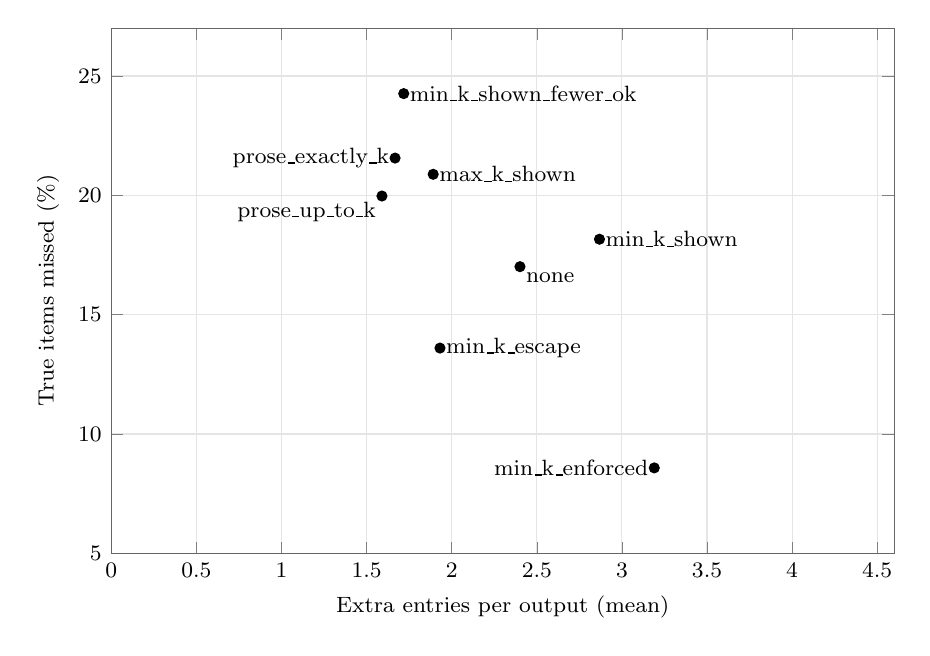
\begin{tikzpicture}
\begin{axis}[scale only axis, width=0.82\columnwidth, height=0.55\columnwidth,
  xmin=0, xmax=4.6, ymin=5, ymax=27, grid=major, grid style={gray!20}, axis line style={black!60},
  xlabel={Extra entries per output (mean)}, ylabel={True items missed (\%)},
  label style={font=\footnotesize}, tick label style={font=\footnotesize}]
\addplot[only marks, mark=*, mark size=1.8pt, color=black] coordinates {(2.401,17.01) (1.590,19.97) (1.667,21.56) (1.891,20.88) (2.868,18.16) (1.718,24.26) (3.190,8.58) (1.931,13.60)};
\node[font=\footnotesize, anchor=north west, inner sep=2pt] at (axis cs:2.401,17.01) {\cnd{none}};
\node[font=\footnotesize, anchor=north east, inner sep=2pt] at (axis cs:1.590,19.97) {\cnd{prose\_up\_to\_k}};
\node[font=\footnotesize, anchor=east, inner sep=2pt] at (axis cs:1.667,21.56) {\cnd{prose\_exactly\_k}};
\node[font=\footnotesize, anchor=west, inner sep=2pt] at (axis cs:1.891,20.88) {\cnd{max\_k\_shown}};
\node[font=\footnotesize, anchor=west, inner sep=2pt] at (axis cs:2.868,18.16) {\cnd{min\_k\_shown}};
\node[font=\footnotesize, anchor=west, inner sep=2pt] at (axis cs:1.718,24.26) {\cnd{min\_k\_shown\_fewer\_ok}};
\node[font=\footnotesize, anchor=east, inner sep=2pt] at (axis cs:3.190,8.58) {\cnd{min\_k\_enforced}};
\node[font=\footnotesize, anchor=west, inner sep=2pt] at (axis cs:1.931,13.60) {\cnd{min\_k\_escape}};
\end{axis}
\end{tikzpicture}

  \caption{Post hoc: mean extra entries per output against the share of true items missed\pre{}, one point per condition, eight GPU models pooled, all documents, $k = 3$ and 5 (the rows of Table~\ref{tab:prf}). Per-model points are in the repository.}
  \label{fig:padmiss}
\end{figure}

\paragraph{Qwen3.5-0.8B read leniently.}
A lenient parser that also takes the list from inside a copy of the schema, and changes none of the outputs the frozen parser already reads, cuts this model's unreadable share from 36.6\% to 9.8\%.
Read this way, it over-counts on 52.8\% of its $n < k$ outputs with no count and on 51.5\% under a shown minimum ($-1.3$ points [$-4.0$, $+1.4$]); on the 622 pairs readable under both conditions, a shown minimum adds 7.4 over-count points [5.0, 9.9] and $+0.23$ entries [$-0.36$, $+0.80$].
Its negative estimate in Table~\ref{tab:permodel} comes from unreadable answers counted as empty lists, not from shorter lists.
Without this model, the seven other GPU models give a main contrast of $+0.80$ entries [0.63, 0.96] against the registered $+0.62$, $+24.7$ over-count points [23.1, 26.4] against $+20.9$, and over-count shares of 35.0\% with no count, 59.8\% under a shown minimum and 89.9\% under an enforced one (\texttt{analysis/posthoc/without\_08b.py}).

\paragraph{How much of the padding is invented.}
Under a shown minimum, on documents with $n < k$, the matcher calls 29.5\% of the GPU models' extra entries invented; spread over the authors' labels in the proportions of the 400-entry check, the share is 23.4\% [20.4, 26.6].
The 7.0\% and 7.3\% of Appendix~\ref{app:checks} are shares of all substantive entries, true items included, over every model and condition.
On the same basis, the hosted models' extra entries are 5.6\% invented.

\paragraph{Documents a model gets right with no count.}
The 34.5\% over-count with no count mixes ordinary extraction error into every absolute rate.
To set it aside, we keep only the (model, document) pairs whose no-count list has exactly $n$ substantive entries (2,275 pairs, 3,884 cells of $k = 3$ or 5), or at most $n$ (4,762 cells), so the no-count over-count is 0 by construction.
On these pairs a shown minimum makes 35.2\% of lists pad, a shown maximum 5.0\%, ``fewer is fine'' 9.6\% and an enforced minimum 83.9\% (Table~\ref{tab:cleanbase}).
Under a shown maximum, which changes the prompt as much, 5.0\% pad, so most of the 35.2\% comes from the minimum itself.
Without Qwen3.5-0.8B the shown-minimum share is 36.7\% (\texttt{analysis/posthoc/clean\_baseline.py}).

\begin{table}[t]
  \centering
  \small
  \setlength{\tabcolsep}{3pt}
  \begin{adjustbox}{max width=\linewidth}
  \begin{tabular}{@{}lrr@{}}
    \toprule
    Condition & No count exactly $n$ & No count at most $n$ \\
    \midrule
    \rows{generated/app_clean_baseline_rows.tex}
    \bottomrule
  \end{tabular}
  \end{adjustbox}
  \caption{Post hoc: over-count (\%, 95\% group-bootstrap interval) on the (model, document) pairs whose no-count list was exactly $n$ entries long or at most $n$, eight GPU models pooled, $n < k$, $k = 3$ and 5. With no count the rate is 0 by construction.}
  \label{tab:cleanbase}
\end{table}

\paragraph{How often real schemas set a list minimum.}
We count list minimums in the 9,542 real-world schemas of JSONSchemaBench \citep{geng2025jsonschemabench} (MIT licence, revision \texttt{5bd0f46}), leaving out fixed-length arrays and tuples such as coordinates (Table~\ref{tab:schemaprev}).
Half the schemas hold an array; 7.7\% put a \texttt{minItems} of at least 1 on a list of strings or objects, and 0.3\% (24 schemas) one of 2 or more, such as a list of players or of interests.
The common schema minimum is therefore 1, the case of the empty-document test (Section~\ref{sec:named}); larger minimums are rare in public schemas.
The function-calling subset (Glaiveai2K) sets none (\texttt{analysis/posthoc/schema\_prevalence.py}).

\begin{table}[t]
  \centering
  \small
  \setlength{\tabcolsep}{3pt}
  \begin{adjustbox}{max width=\linewidth}
  \begin{tabular}{@{}lrrrrr@{}}
    \toprule
    Subset & Schemas & Array \% & Min $\geq 1$, list \% & Min $\geq 2$ \% & Min $\geq 2$, list \% \\
    \midrule
    \rows{generated/app_schema_prevalence_rows.tex}
    \bottomrule
  \end{tabular}
  \end{adjustbox}
  \caption{Post hoc: list minimums in JSONSchemaBench, share of schemas. Array: any array. Min $\geq 1$, list: an open array of strings or objects with \texttt{minItems} $\geq 1$. Min $\geq 2$: any open array with \texttt{minItems} $\geq 2$; list: of strings or objects. Open arrays exclude fixed-length arrays (\texttt{minItems} = \texttt{maxItems}) and tuples.}
  \label{tab:schemaprev}
\end{table}

\paragraph{Examples.}
One over-counting output per set under a shown minimum, on a document with $1 \leq n < k$ and with at most six short entries, chosen by a fixed hash rule, not by hand.
The labels are the matcher's; in the emails example it swaps entries 1 and 2, though the number of extra entries is right.

\paragraph{Meetings.} Olmo 3.1 32B, $k = 3$, $n = 1$: 3 entries, 2 extra.
Asked for: Next steps that a meeting participant will take after this meeting, one per job. One short sentence each. Not decisions, and not instructions they will receive.
True items: ``The group will find out if the kinetic energy component can provide enough energy.''.
Output: (1) ``Check with the R\&D department to see if the kinetic metal technology can provide sufficient energy for the remote.'' [true item]; (2) ``Consult with the R\&D department regarding the readiness of the kinetic energy product for market.'' [split true item, extra]; (3) ``Gather and share pictures of the device cases with the Industrial Designer for material identification (titanium vs. plastic).'' [wrong kind, extra].

\paragraph{Emails.} Olmo 3.1 32B, $k = 3$, $n = 2$: 4 entries, 2 extra.
Asked for: Things the sender asks the recipient to do or to provide, one per thing asked. Copy each request as written in the email.
True items: ``What do we need to do to get this''; ``how soon can it be granted?''.
Output: (1) ``Everyone in risk management needs to get access to EOL bridge monitor and reports.'' [true item]; (2) ``What do we need to do to get this access?'' [split true item, extra]; (3) ``How soon can the access be granted?'' [true item]; (4) ``We need this access by Thursday to be prepared for testing.'' [wrong kind, extra].

\paragraph{Receipts.} Qwen3.5-9B, $k = 3$, $n = 1$: 3 entries, 2 extra.
Asked for: Names of the items purchased on this receipt, one entry per item, copied as printed.
True items: ``ALMOND CHOCO CREAM CHEESE''.
Output: (1) ``ALMOND CHOCO CREAM CHEESE'' [true item]; (2) ``SUB TOTAL'' [wrong kind, extra]; (3) ``GRAND TOTAL'' [wrong kind, extra].

\paragraph{Job-ad skills.} Olmo 3.1 32B, $k = 5$, $n = 1$: 5 entries, 4 extra.
Asked for: Skills, abilities and duties the job ad mentions, copied as written. Not tools, technologies, fields of knowledge, languages or certificates.
True items: ``running with a full stack development''.
Output: (1) ``running full stack development'' [true item]; (2) ``Java'' [wrong kind, extra]; (3) ``Python'' [wrong kind, extra]; (4) ``React JS'' [wrong kind, extra]; (5) ``Redux'' [wrong kind, extra].

\paragraph{Clinical.} Ministral 3 14B, $k = 5$, $n = 3$: 5 entries, 2 extra.
Asked for: Medications or drugs, by name or by class, mentioned as given to or taken by the patient, copied as written.
True items: ``ACE inhibitor''; ``diuretic''; ``$\beta$-blocker''.
Output: (1) ``ACE inhibitor'' [true item]; (2) ``diuretic'' [true item]; (3) ``low-dose $\beta$-blocker'' [true item]; (4) ``coronary angiography contrast agent (if applicable)'' [invented, extra]; (5) ``endomyocardial biopsy procedural sedation/anesthesia (if applicable)'' [invented, extra].

\paragraph{Reviews.} Qwen3.5-2B, $k = 5$, $n = 1$: 5 entries, 4 extra.
Asked for: Features or aspects of the product or service that the reviewer gives an opinion on, copied as written.
A short hotel review from the restricted reviews set (no review text is reproduced here). The reviewer calls the hotel a hidden gem of its city, says they had expected an ordinary chain hotel, says it beat every hotel they had used in a long time, and praises the staff. The answer list holds one item: the staff.

The model's list has five entries. Four copy short phrases from the review that name the hotel or praise it in general (its headline, the chain it was expected to resemble, the comparison with other hotels); the matcher calls all four real text of the wrong kind, so all four are extra. The fifth, praise of the staff, is the one true item. (Paraphrased: review text is not redistributed.)

\paragraph{Job-ad knowledge.} Gemma 4 31B, $k = 5$, $n = 2$: 5 entries, 3 extra.
Asked for: Tools, technologies, fields of knowledge, languages and certificates the job ad mentions, copied as written. Not abilities or duties.
True items: ``science''; ``pharmaceutical production''.
Output: (1) ``science education'' [true item]; (2) ``pharmaceutical production'' [true item]; (3) ``management experience'' [wrong kind, extra]; (4) ``communication skills'' [wrong kind, extra]; (5) ``collaboration skills'' [wrong kind, extra].

\paragraph{Wikipedia people.} Qwen3.5-2B, $k = 5$, $n = 2$: 3 entries, 1 extra.
Asked for: Names of people mentioned in the text, copied as written.
True items: ``Stamatiad''; ``Emil Gârleanu''.
Output: (1) ``Stamatiad'' [true item]; (2) ``Emil Gârleanu'' [true item]; (3) ``Romanian Writers ' Society (SSR)'' [wrong kind, extra].

\paragraph{Novel quotes.} gpt-oss-20b, $k = 5$, $n = 3$: 5 entries, 2 extra.
Asked for: Direct speech quoted in the text, copied word for word.
True items: ``After what happened at Vevey, I think I may certainly call upon them,''; ``If, after what happens-{}-at Vevey and everywhere-{}-you desire to keep up the acquaintance, you are very welcome. Of course a man may know everyone. Men are welcome to the privilege!''; ``Pray what is it that happens-{}-here, for instance?''.
Output: (1) ``After what happened at Vevey'' [true item]; (2) ``I think I may certainly call upon them,'' [split true item, extra]; (3) ``If, after what happens-{}-at Vevey and everywhere-{}-you desire to keep up the acquaintance, you are very welcome.'' [true item]; (4) ``Of course a man may know everyone. Men are welcome to the privilege!'' [split true item, extra]; (5) ``Pray what is it that happens-{}-here, for instance?'' [true item].



\section{Pilot stop rules}
\label{app:stoprules}

Both pilot stop rules on over-count say go: on pilot documents, $n < k$, $k = 3$ and 5, pooled over the three pilot models, \cnd{min\_k\_shown} minus \cnd{none} was $+34.4$ points [28.1, 40.8] (Qwen3.5-9B 30.0, Ministral 3 14B 13.3, Gemma 4 31B 60.0) and \cnd{min\_k\_shown} minus \cnd{max\_k\_shown} $+34.2$ [28.3, 40.3].
The third stop rule, the blind check at the registered threshold of 85\%, passes (Appendix~\ref{app:key}).
The stop-rule simulation, rerun with the pilot's floor rates (600 simulations), stops at a true gap of 0 points with probability 0.68 to 0.80 and goes at a true gap of 10 points with probability 0.67 to 0.82 across floors of 15 to 78\%.
